\documentclass[11pt]{article}
\usepackage{graphicx}
\usepackage[margin=1in]{geometry}
\usepackage{mathtools}
\usepackage{hyperref}
\linespread{1.5}
\title{\textbf{Self Organizing Maps \& CUDA}}
\author{Doug Woodward}
\date{}
\begin{document}

\maketitle
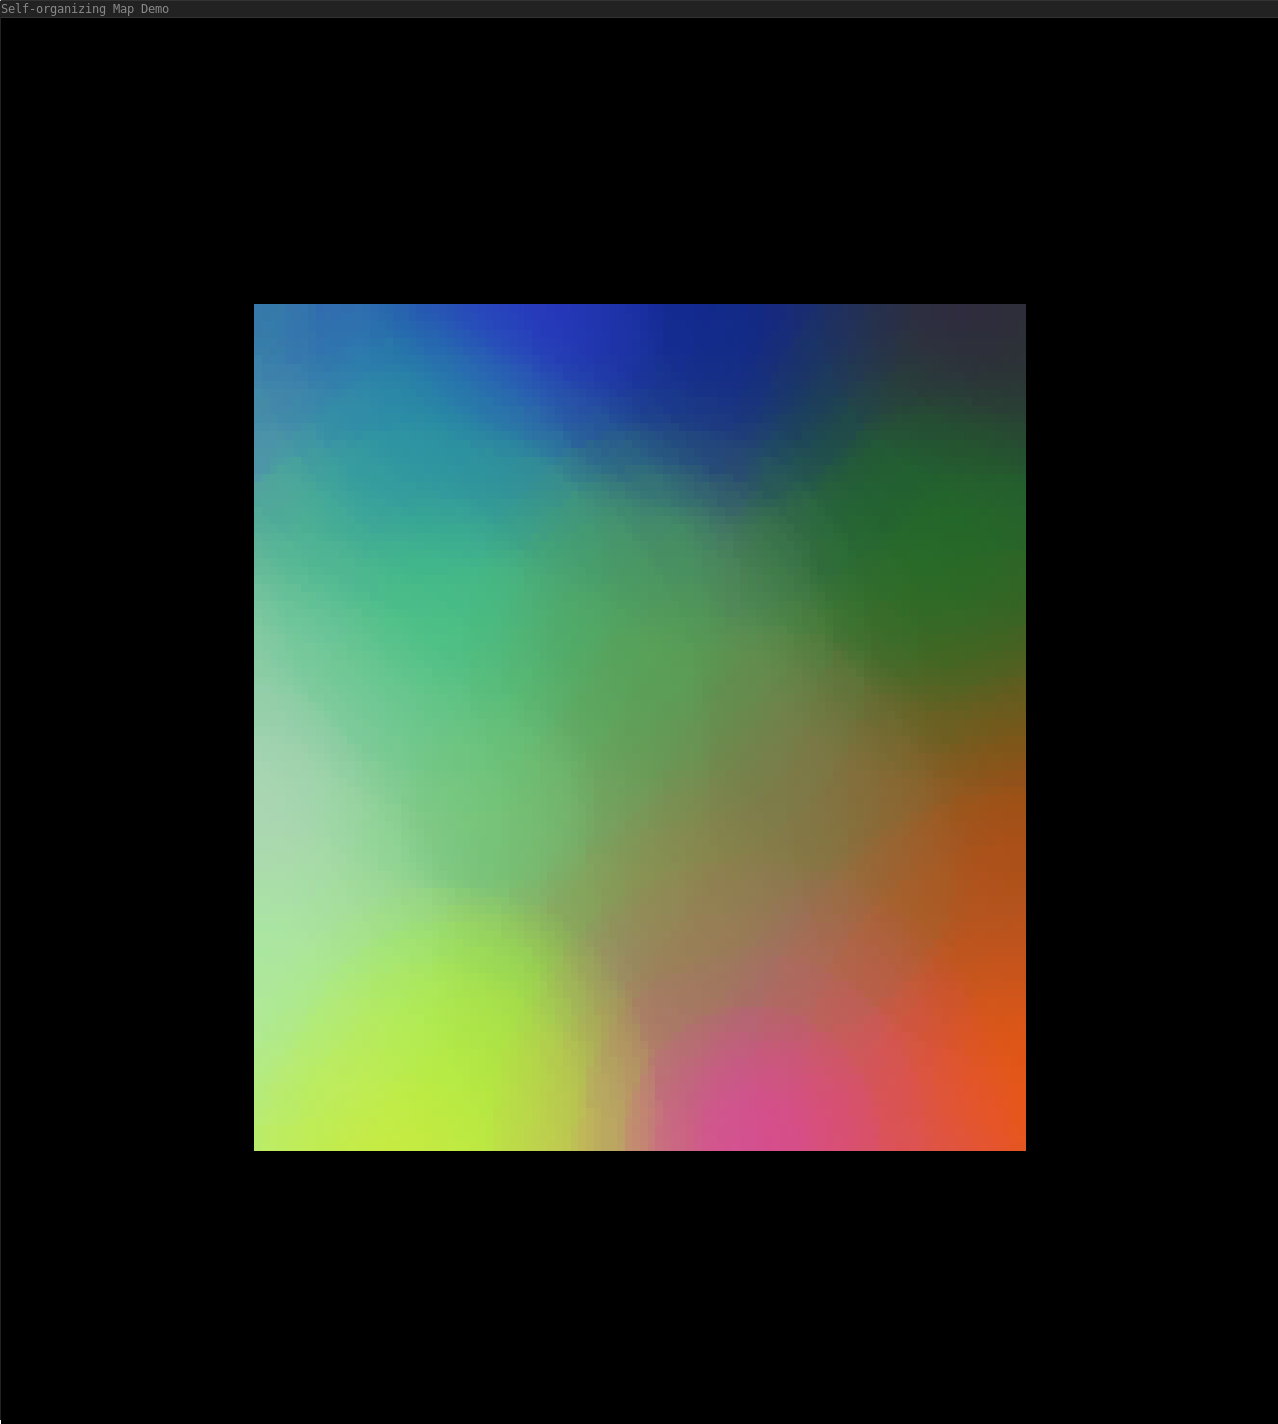
\includegraphics[scale=.15]{title}
\section{Introduction}

Self Organizing Maps are a type of clustering, unsupervised neural network well suited to visually displaying information that exists in higher dimensional spaces down into two and three dimensional space such that a human observer can interpret it intuitively. Self Organzing maps preserve the topological relationships of high dimensional data when compressing down into lower dimensional space. SOMs are frequently used in meteorology, oceanography, prioritization, and even in the creation of artwork - an unexpected use to be sure, but one that even this project gives credit to in the distributions of colors when adjusting parameters. This paper seeks to explore the parallelization of a SOM algorithm using CUDA to leverage the high throughput capability of GPUs.

In this paper, the data the SOM is trained on is fairly trivial, RGB color points - three dimensional data that will be clustered in two dimensional space. However, the algorithm and implementation herein can be converted with minimal effort to handle more complex data - for example, RGBA values or even data points with hundreds of attributes. The key requirement is that there exists a method of distance calculation between two points.
\section{SOM Implementation}
Implementing a SOM can be broken down into the following steps:
\begin{enumerate}
\item{Initialization}
\item{Sampling}
\item{Matching}
\item{Updating}
\item{Repeat}
\end{enumerate}
\subsection{Initialization}
The initialization of a SOM can have a signifigant influence on the end result and the time taken to train the algorithm. In this project, the data is intialized as a N*M matrix of RGB points where the RGB values of each points are generated randomly. The intialized, untrained map is below.

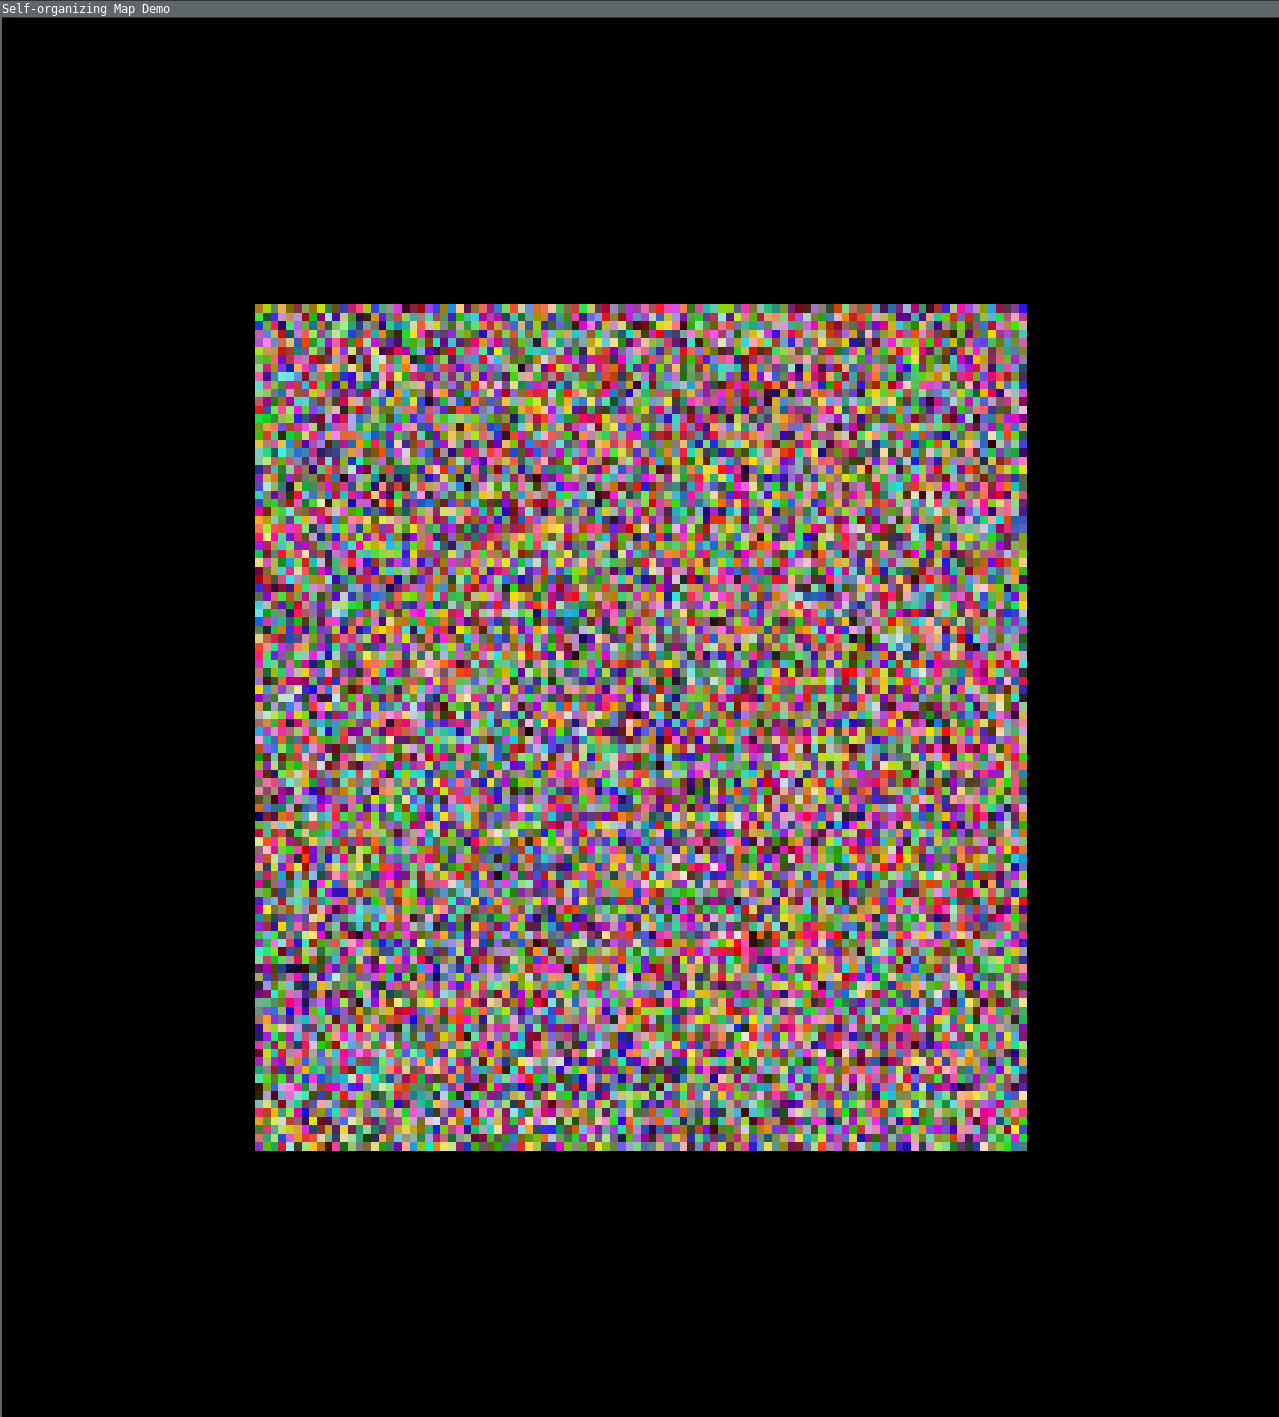
\includegraphics[scale=.15]{cuda_som_init}

Each time the map is intialized the points are assigned RGB values at random, resulting in even the same training data set producing differing outputs in the overall arrangement. That is not to say the clustering is any different, nor does the relative arrangement of clusters change, but the entire SOM may be rotated or transformed as below. 

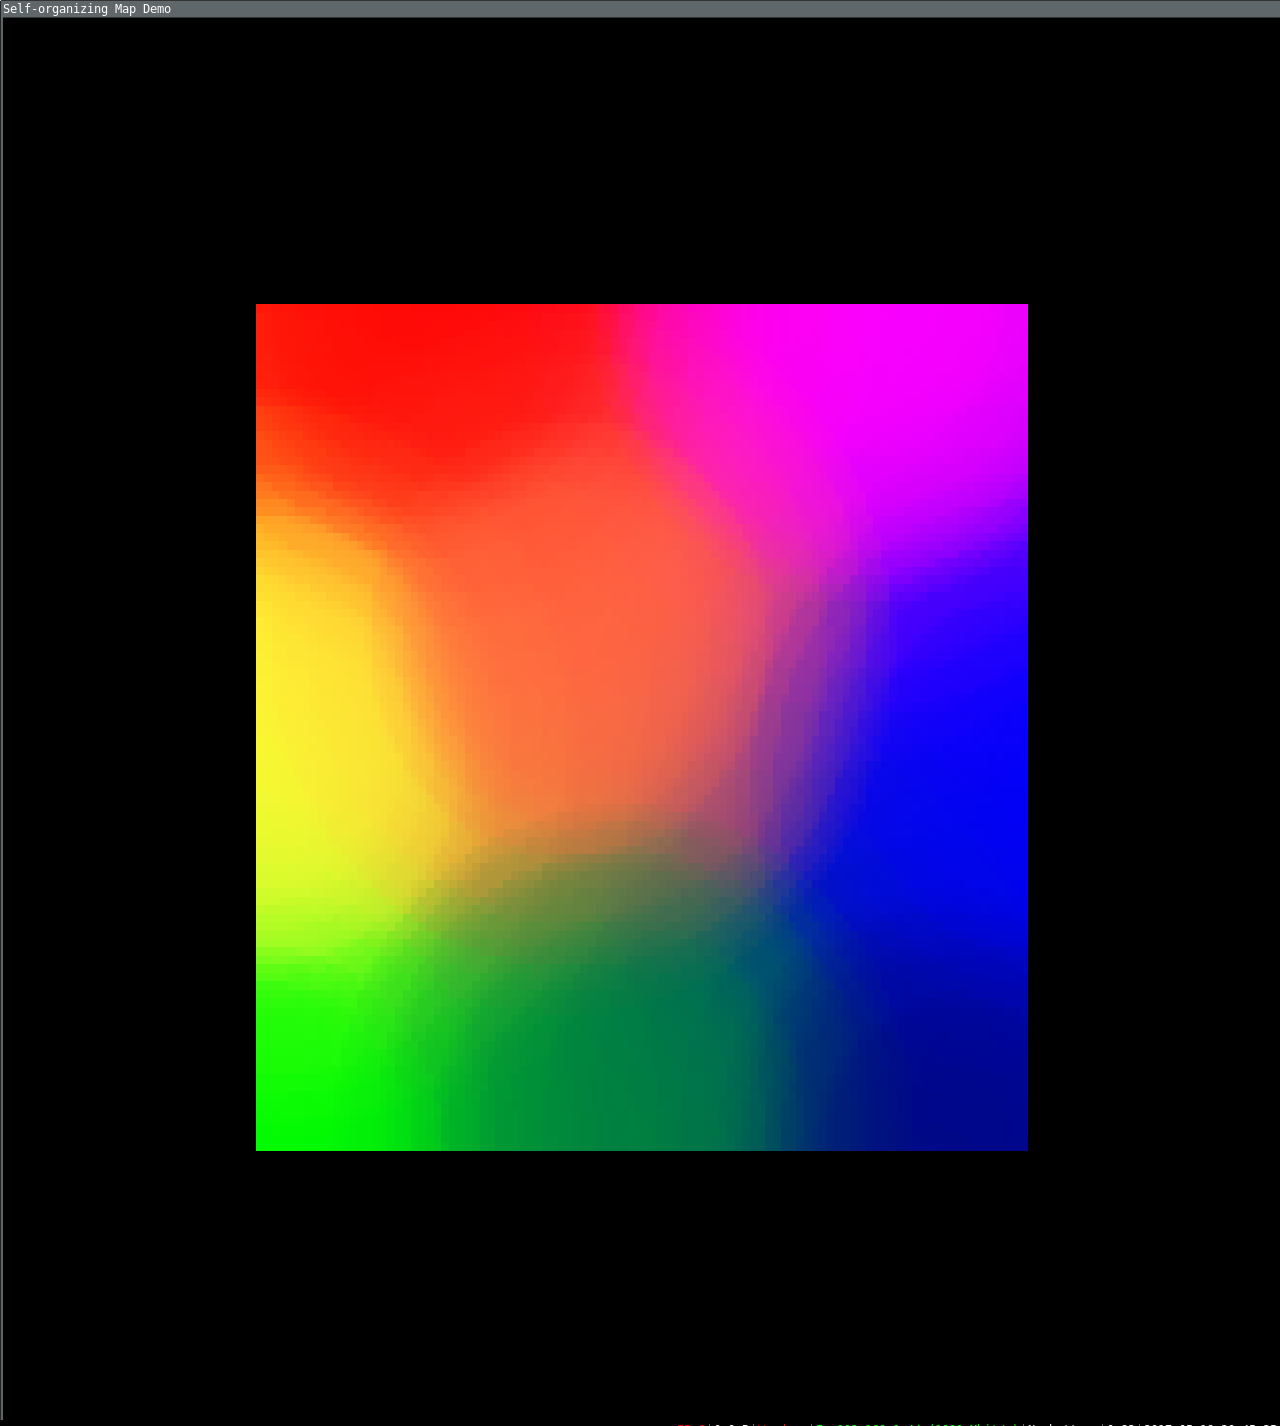
\includegraphics[scale=.15]{output1}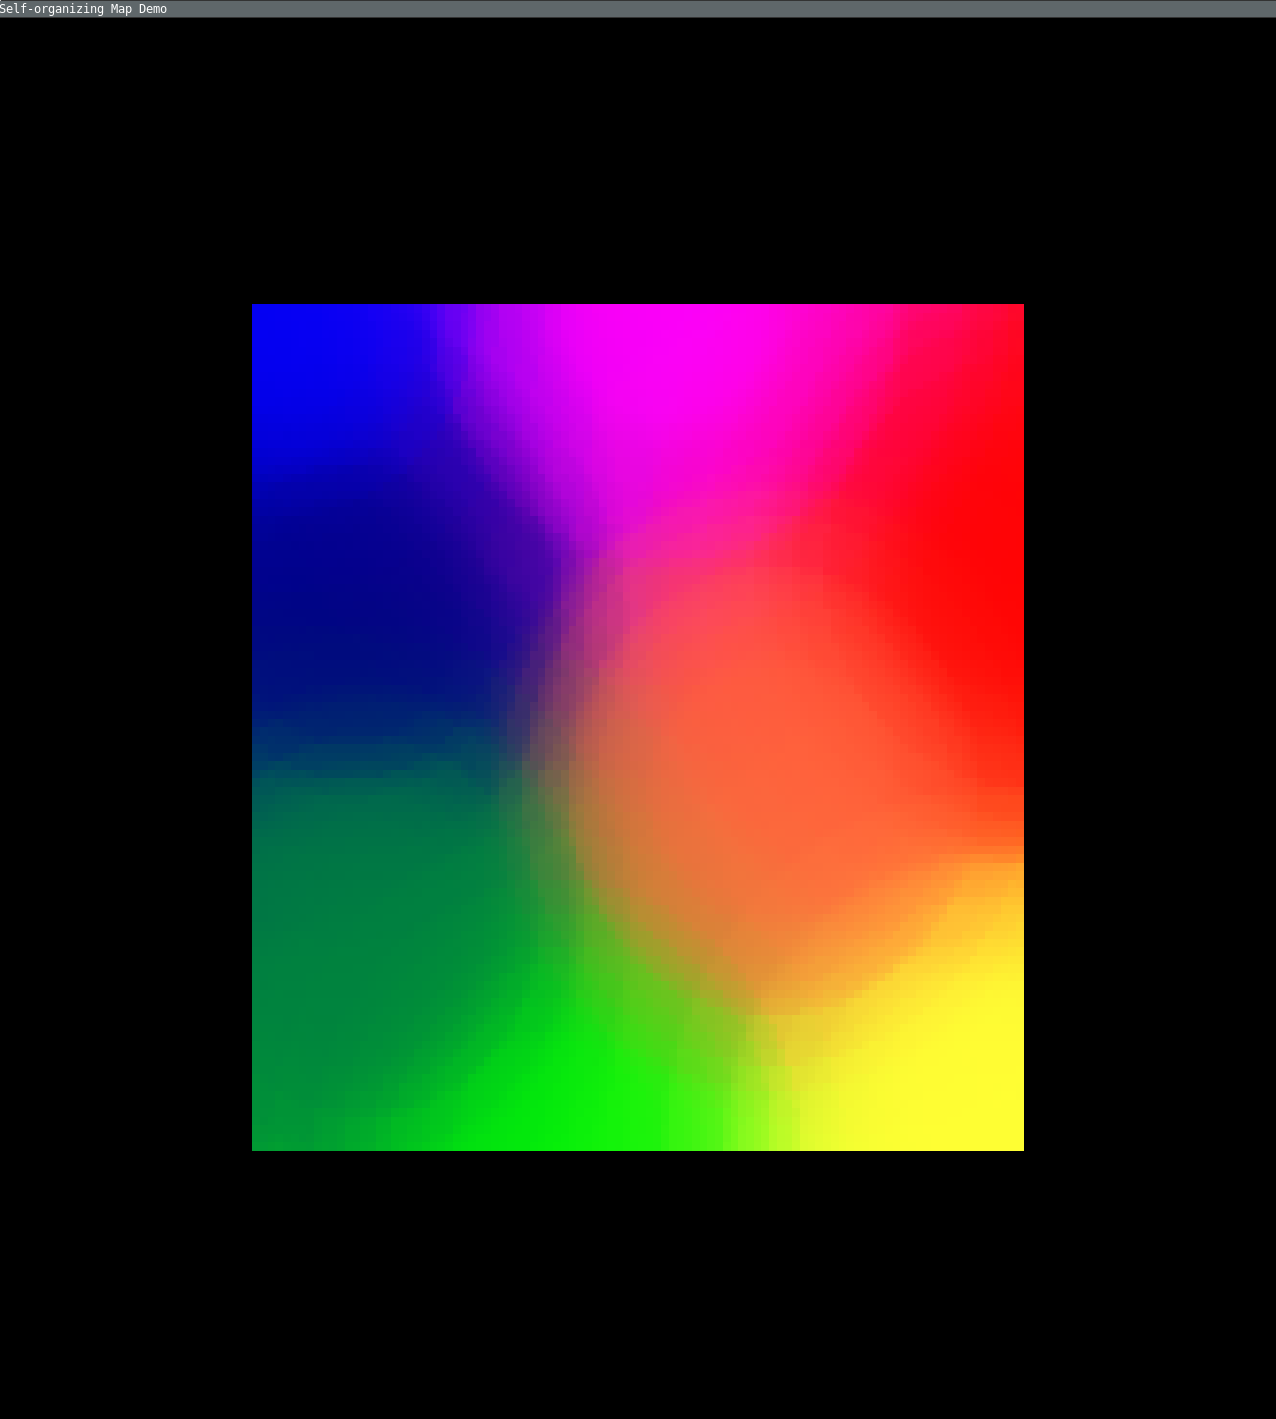
\includegraphics[scale=.1505]{output2}

This variance is explained by the algorithm selecting the closest match for each input data point and adjusting the surrounding weights accordingly, with random intialization of the map, the closest point to say Dark Blue, could be anywhere on the map to start, top left, bottom right etc. However, orange always clusters to the center as the map retains the topological relationships between clusters in lower dimensional space.

\subsection{Sampling}

The sampling step is a fairly straightforward process, from the training data, a point is selected at random to be input into the map. Of note here, the random selection has no more bearing on the final result than the random initialization, it may effect the rotation or transformation but can not effect the topological relationships.

\subsection{Matching}

Here, the need for a distance formula specific to the data set arises. Within the scope of this paper, a simple Euclidean Distance formula is used: \begin{math}\sqrt{\sum\limits_{i=0}^{i=n} ({p^1_i}-{p^2_i})^2} \end{math}  where \(p^1\) and \(p^2\) are two RGB color points. For other data sets, more complex distance formulae may be neccesary. Once the best match is chosen, the algotrithm proceeds to the next step. Because of the need to process the same simple equation on many points when each individual calculation has no bearing on th others, this section of the algorithm was targeted for parallelization.t

\subsection{Updating}

Following the selection of the best matching point, the points surrounding the best match must be updated as well, with the magnitude of the decrease scaling inversly with the distance from a node and also influenced by the learning rate, which typically decreases over the life of the training. To have the radius of influence shrink with time an exponential decay function is used. \begin{math}\sigma_0exp(-t/\lambda) \end{math} where \(\sigma_0\) is the half the width of the map, \(t\) is the time step, and \(\lambda\) is the learning rate which is equivalent to the current number of iterations over the log of half the width of the map. 

\subsection{Repeating}

The algorithm repeats the above steps until some break condition is met. For this project, the break conditions are that set are a certain number of iterations, 1000, or if the total change induced in the map by a data point is less than 0.1.

\section{Parallelization with CUDA}

In applying parallelization to the algorithm, the matching step was the most viable candidate for optimization. Adjusting the code to accomodate a Cuda kernel call required more effort than dropping an OpenMP section into the code. One notable restriction of CUDA is the lack of more sophisticated data structures, which limits the ability to apply an object oriented approach to a CUDA program. This also meant that the nested std::vector data structures employed needed to be flattened into a one dimesional array of doubles to be used by the CUDA kernel call. This meant that the entire matrix became an \(N \times M3\) length pointer and the vector of distances for each node in a comparison became an \(N*M\) array. Because of this length mismatch, the indexing required some adjustment based on the thread id such that the index for the flattened map was multiplied by 3 during the interior loop of the kernel over RGB values.

Unfortunatlely, there was no speedup realized by the implementation of CUDA in this algorithm. That is not to say that a Self Organizing Map can not be parallelized to take advantage of GPU processing power, rather that the implementation of the SOM in this project was an ill suited match for it. The results of runs in parallel and serial execution are shown below with a number of different map sizes.




\begin{table}[!htbp]
\centering
\begin{tabular}{|c|c|c|c|c|}
\hline
	Size & Serial & Parallel & Speedup & Efficiency\\
\hline
	 100x100 & 8.396 & 8.943 &  &\\
\hline
	100 x 10 & 10.10 & 10.266 & &\\
\hline
	0.012676 &  0.006117 & 2.05 & &\\
\hline
	 0.012174 & 0.007373 & & &\\
\hline
	0.012163 & 0.0069 & & &\\
\hline
\end{tabular}
\end{table}

Amdahl's law was not employed here because the only section that was parallelized and measured was the traversal - in which either all of it or none of it was run in parallel, and the use of recursion renders it difficult to break down the code into serial and parallel by percentage.


\section{Conclusion}
Parallelization is a powerful technique and one that can yield great gains --- however, not all applications are well suited for it. A generalization can be drawn here that sections of code that require writing to an object or memory are ill-suited for parallelization. However, searching some data structure and only accessing memory for reads presents an excellent potential area for the use of parallelization. 

\section{Code}

Code can be found at \texttt{\href{https://github.com/rugggg/CADS/tree/master/CS540/nBody}{https://github.com/rugggg/CADS/tree/master/CS540/nBody}}

\begin{thebibliography}{9}
\bibitem{nasa} 
How Many Solar System Bodies
\\\texttt{https://ssd.jpl.nasa.gov/?body\_count}
\textit{NASA JPL}. 
 
\bibitem{openmp} 
OpenMP
\texttt{http://www.openmp.org/}
[\textit{OpenMP 4.5 Specifications}]. 
Annalen der Physik, 322(10):891–921, 1905.
 
\bibitem{barnes-hut} 
The Barnes-Hut Algorithm
\textit{Tom Ventimiglia \& Kevin Wayne}
\\\texttt{http://arborjs.org/docs/barnes-hut}

\bibitem{barnes-hut} 
The Barnes-Hut Algorithm
\textit{Tom Ventimiglia \& Kevin Wayne}
\\\texttt{http://arborjs.org/docs/barnes-hut}
\end{thebibliography}

\end{document}